% Figure from MATH 591 notes, section 49. Compile with the notes preamble.
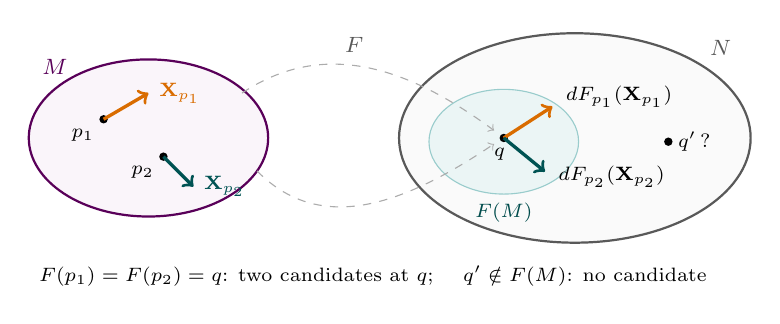
\begin{tikzpicture}[scale=0.95]
\draw[thick, violet!70!black, fill=violet!4] (0,0) ellipse (1.6 and 1.05);
\node[violet!70!black, font=\footnotesize] at (-1.25,0.95) {$M$};
\fill (-0.60,0.25) circle (1.6pt) node[below left, font=\scriptsize] {$p_1$};
\fill (0.20,-0.25) circle (1.6pt) node[below left, font=\scriptsize] {$p_2$};
\draw[->, very thick, orange!85!black] (-0.60,0.25) -- ++(0.6,0.35) node[right, font=\scriptsize] {$\mathbf{X}_{p_1}$};
\draw[->, very thick, teal!65!black] (0.20,-0.25) -- ++(0.4,-0.4) node[right, font=\scriptsize] {$\mathbf{X}_{p_2}$};
\draw[thick, gray!70!black, fill=gray!4] (5.7,0) ellipse (2.35 and 1.4);
\node[gray!70!black, font=\footnotesize] at (7.65,1.2) {$N$};
\draw[teal!40, fill=teal!8] (4.75,-0.05) ellipse (1.0 and 0.7);
\node[teal!60!black, font=\scriptsize] at (4.75,-1.0) {$F(M)$};
\fill (4.75,0.00) circle (1.6pt) node[below, xshift=-1.5pt, font=\scriptsize] {$q$};
\draw[->, very thick, orange!85!black] (4.75,0.00) -- ++(0.65,0.42);
\draw[->, very thick, teal!65!black] (4.75,0.00) -- ++(0.55,-0.45);
\node[font=\scriptsize, anchor=west] at (5.45,0.55) {$dF_{p_1}(\mathbf{X}_{p_1})$};
\node[font=\scriptsize, anchor=west] at (5.35,-0.52) {$dF_{p_2}(\mathbf{X}_{p_2})$};
\fill (6.95,-0.05) circle (1.6pt) node[right, font=\scriptsize] {$q'$\,?};
\draw[->, dashed, gray!65] (1.25,0.6) .. controls (2.3,1.3) and (3.4,1.0) .. (4.62,0.1);
\draw[->, dashed, gray!65] (1.45,-0.44) .. controls (2.3,-1.3) and (3.4,-0.9) .. (4.62,-0.08);
\node[gray!70!black, font=\footnotesize] at (2.75,1.25) {$F$};
\node[font=\scriptsize, align=center] at (3.0,-1.85) {$F(p_1) = F(p_2) = q$: two candidates at $q$; \quad $q' \notin F(M)$: no candidate};
\end{tikzpicture}
